\chapter{Multimodal Inference of Mind SCAIN}
\par
本論文では,行動情報と発話情報の両方を活用し,信念と欲求の推定を行うシステムMultimodal Inference of Mind SCAIN (MIoM SCAIN)を提案する.MIoM SCAINは,人間の行動,発話および人間が存在する環境の状態を基に信念と欲求を推定する.行動情報と発話情報の両方を信念と欲求の推定に活用することで,発話による行動の解釈の変化や行動による発話の解釈の変化を捉え,行動情報と発話情報の相互作用を考慮して信念と欲求を推定する.

\par
MIoM SCAINは,環境の状態や人間の心的状態を部分的に観測可能なマルコフ決定過程として表す.また,信念と欲求の推定値はそれぞれの候補に対し尤度が与えられたパーティクルフィルタとして表され,信念と欲求の組み合わせを一意に決定するのではなく同時に複数保持し,時刻が経過する度に各パーティクルの尤度を更新していく.各時刻における人間の信念や行動,発話および人間が存在する環境の状態をベイズ推論に適用し,環境中で人間が観測できていない部分についての信念と欲求を逐次的に推定する.


\section{アルゴリズム}

\par
MIoM SCAINにおける推定処理の流れをを図\ref{fig:sys_arc}に示す.
\begin{figure}[htbp]
  \begin{center}
    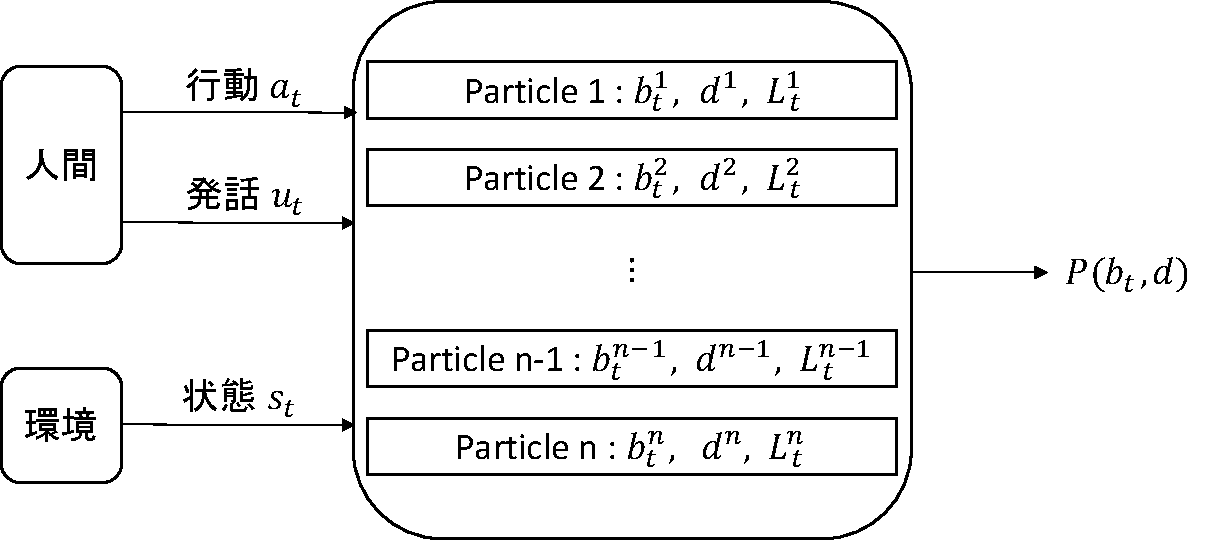
\includegraphics[scale=0.7]{./bt1.pdf}
    \caption{MIoM SCAINによる推定処理}
    \label{fig:sys_arc}
  \end{center}
\end{figure}
図\ref{fig:sys_arc}に示すように,MIoM SCAINは時刻$t$における人間の行動$a_t$,発話$u_t$および環境の状態$s_t$から信念と欲求の確率を出力する.MIoM SCAINは信念$b_t$と欲求$d$の組み合わせとその尤度$L$を持つパーティクルフィルタとして表現され,$a_t,u_t,s_t$とパーティクル$k$が持つ信念$b_t^k$と欲求$d^k$を基に尤度$L^k$が更新される.尤度$L^k$は次のように表すことができる.
\begin{equation}
  \begin{split}
  \label{pf}
  L^k=P(b_t^k,d^k|s_{1:t},a_{1:t-1},u_{1:t-1})
  \end{split}
\end{equation}
ここで,$u_{1:t-1}$は,時刻$1$から時刻$t-1$までの人間の発話履歴,$P(b_t,d|s_{1:t},a_{1:t-1},u_{1:t-1})$は,$s_{1:t},a_{1:t-1}およびu_{1:t-1}$から計算される$b_t$と$d$の確率である.

\par
図\ref{fig:miom}にMIoM SCAINにおけるベイズ推論を表現するベイジアンネットワークを示す.$s_t$,$a_t$および$u_t$は観測値,$o_t$,$b_t$および$d$は確率変数として扱う.
\begin{figure}[htbp]
  \begin{center}
    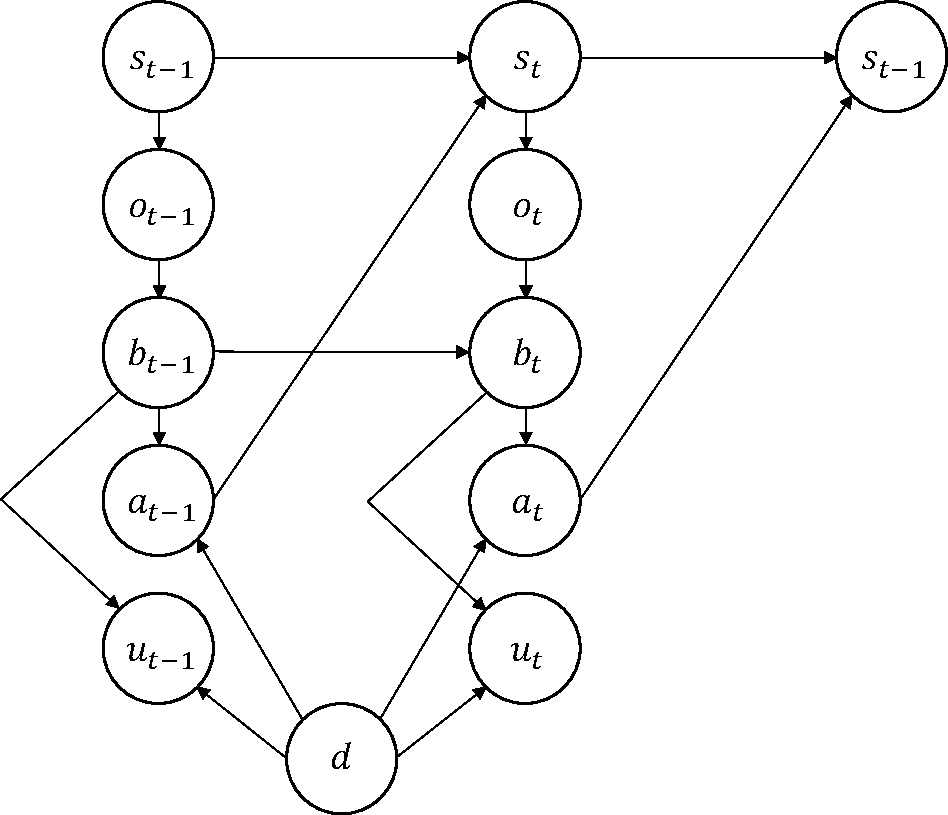
\includegraphics[scale=0.73]{./miom.pdf}
    \caption{MIoM SCAINにおけるベイズ推論を表現するベイジアンネットワーク}
    \label{fig:miom}
  \end{center}
\end{figure}
MIoM SCAINにおけるベイズ推論では,BToMと同様に時刻$t$における環境の状態$s_{t}$を基に人間の観測状況$o_{t}$が決まる.また,$o_{t}$を基に人間の信念$b_{t}$が決まり,$b_{t}$と人間の欲求$d$から人間の行動$a_{t}$が決まる.それに加え,MIoM SCAINでは$b_t$と$d$から人間の発話$u_t$が決まる.また$a_{t}$が起こることにより,環境の状態は$s_{t+1}$に変化し,人間の観測状況,信念,行動および発話が再び計算される.MIoM SCAINでは各パーティクルの尤度である式(\ref{pf})を計算することを目的としている.ベイズの定理と図\ref{fig:miom}における変数間の条件付き独立性より,式(\ref{eq_miom})が成り立つ.
\begin{equation}
  \begin{split}
  \label{eq_miom}
  L^k&=P(b_t^k,d^k|s_{1:t},a_{1:t-1},u_{1:t-1})\\
  &\propto P(b_t^k,d^k,s_{1:t},a_{1:t-1},u_{1:t-1})\\
  &= \sum_{b_{t-1}^k,o_t}P(b_t^k,d^k,s_{1:t},a_{1:t-1},u_{1:t-1},b_{t-1}^k,o_t)\\
  &= \sum_{b_{t-1}^k,o_t}P(b_t^k|d^k,s_{1:t},a_{1:t-1},u_{1:t-1},b_{t-1}^k,o_t)\cdot P(d^k,s_{1:t},a_{1:t-1},u_{1:t-1},b_{t-1}^k,o_t)\\
  &= \sum_{b_{t-1}^k,o_t}P(b_t^k|b_{t-1}^k,o_t)\cdot P(o_t|d^k,s_{1:t},a_{1:t-1},u_{1:t-1},b_{t-1}^k)\\
  &\hspace{5cm} \cdot P(d^k,s_{1:t},a_{1:t-1},u_{1:t-1},b_{t-1}^k)\\
  &= \sum_{b_{t-1}^k,o_t}P(b_t^k|b_{t-1}^k,o_t)\cdot P(o_t|s_t)\cdot P(s_t|s_{t-1},a_{t-1})\\
  &\hspace{3cm} \cdot P(a_{t-1}|b_{t-1}^k,d^k)\cdot P(u_{t-1}|b_{t-1}^k,d^k)\cdot P(b_{t-1}^k,d^k,s_{1:t-1},a_{1:t-2},u_{1:t-2})\\
  &\propto \sum_{b_{t-1}^k,o_t}P(b_t^k|b_{t-1}^k,o_t)\cdot P(o_t|s_t)\cdot P(s_t|s_{t-1},a_{t-1})\\
  &\hspace{3cm} \cdot P(a_{t-1}|b_{t-1}^k,d^k)\cdot P(u_{t-1}|b_{t-1}^k,d^k)\cdot P(b_{t-1}^k,d^k|s_{1:t-1},a_{1:t-2},u_{1:t-2})\\
  \end{split}
\end{equation}
ここで,$P(b_t^k|b_{t-1}^k,o_t)$は人間の観測状況$o_t$によってパーティクル$k$の信念$b_t^k$が更新される確率,$P(o_t|s_t)$は環境の状態$s_t$において人間が観測状況$o_t$を得る確率,$P(s_t|s_{t-1},a_{t-1})$は環境の状態$s_{t-1}$において人間が行動$a_{t-1}$を起こした時に環境の状態が$s_{t}$になる確率,$P(a_{t-1}|b_{t-1}^k,d^k)$はパーティクル$k$が信念$b_{t-1}^k$,欲求$d^k$を持つ時に行動$a_{t-1}$を起こす確率,$P(u_{t-1}|b_{t-1}^k,d^k)$はパーティクル$k$が信念$b_{t-1}^k$,欲求$d^k$を持っている時に発話$u_t$を起こす確率,$P(b_{t-1}^k,d^k|s_{1:t-1},a_{1:t-2},u_{1:t-2})$は時刻$t-1$におけるパーティクル$k$の尤度である.式(\ref{eq_miom})より,$L^k$は初期値$P(b_1,d|s_1,a_0,u_0)$を決めて順次更新する計算により求めることができる.
% また,$L^k$は$P(b_t^k|b_{t-1}^k,o_t)$,$P(o_t|s_t)$,$P(s_t|s_{t-1},a_{t-1})$,$P(a_{t-1}|b_{t-1}^k,d^k)$および$(u_{t-1}|b_{t-1}^k,d^k)$の乗算として表すことができる.

\section{実装}
\par
% それぞれの生起確率がどのように計算されるかを記載
MIoM SCAINでは,式(\ref{eq_miom})に示すように各パーティクルにおいて$P(b_t^k|b_{t-1}^k,o_t)\cdot P(o_t|s_t)$,$P(s_t|s_{t-1},a_{t-1})$,$P(a_{t-1}|b_{t-1}^k,d^k)$および$P(u_{t-1}|b_{t-1}^k,d^k)$を計算し,前時刻のパーティクルの尤度を乗算することにより,信念$b_t^k$と欲求$d^k$の尤度を更新する.

\par
最初に,$P(b_t^k|b_{t-1}^k,o_t)\cdot P(o_t|s_t)$の計算方法について説明する.$P(b_t^k|b_{t-1}^k,o_t)\cdot P(o_t|s_t)$は,式(\ref{calc_b_o})により信念$b_t^k$と観測状況$o_t$を比較し計算する.
\begin{equation}
  \begin{split}
  \label{calc_b_o}
  P(b_t^k|b_{t-1}^k,o_t)\cdot P(o_t|s_t)=
  \begin{cases}
    1 & (b_t^kとo_tが一致する時) \\
    0 & (b_t^kとo_tが一致しない時)
  \end{cases}
  \end{split}
\end{equation}

\par
次に$P(s_t|s_{t-1},a_{t-1})$の計算方法について説明する.$P(s_t|s_{t-1},a_{t-1})$は,式(\ref{calc_s})により計算される.
\begin{equation}
  \begin{split}
  \label{calc_s}
  P(s_t|s_{t-1},a_{t-1})=
  \begin{cases}
    1 & (s_t=T(s_{t-1},a_{t-1})) \\
    0 & (otherwise)
  \end{cases}
  \end{split}
\end{equation}
ここで,関数$T(s_{t-1},a_{t-1})$は環境の状態$s_{t-1}$および行動$a_{t-1}$を入力とし,次の環境の状態$s_t$を出力する関数である.

\par
次に$P(a_{t-1}|b_{t-1}^k,d^k)$の計算方法について説明する.$P(a_{t-1}|b_{t-1}^k,d^k)$は式(\ref{calc_a})により計算される.
\begin{equation}
  \begin{split}
  \label{calc_a}
  P(a_{t-1}|b_{t-1}^k,d^k)=\mathrm{softmax}(Q_{t-1},\delta)
  \end{split}
\end{equation}
ここで,$Q_{t-1}$は行動$a_{t-1}$の予測報酬,$\delta$は$P(a_{t-1}|b_{t-1}^k,d^k)$への予測報酬$Q_{t-1}$の寄与を調整する変数である.

\par
最後に$P(u_{t-1}|b_{t-1}^k,d^k)$の計算方法について説明する.$P(u_{t-1}|b_{t-1}^k,d^k)$は,式(\ref{calc_u})により計算される.
\begin{equation}
  \begin{split}
  \label{calc_u}
  P(u_{t-1}|b_{t-1}^k,d^k)\propto \sum_{i=1}^n(\alpha+\beta_p)\cdot\mathrm{similarity}(u_{t-1},g_i)
  \end{split}
\end{equation}
ここで,$g_i$は信念$b_{t-1}^k$または欲求$d^k$になり得る環境中の対象物,関数$\mathrm{similarity}(u_{t-1},g_i)$は発話$u_{t-1}$および環境中の対象物$g_i$を入力とし,Word2Vec \cite{mikolov2013efficient}により発話$u_{t-1}$を分散表現に変換した後,信念$b_{t-1}^k$または欲求$d^k$になり得る環境中の対象物$g_i$との類似度を出力する関数,$\alpha$は環境中の対象物$g$が信念$b_{t-1}^k$にあたる場合において$\mathrm{similarity}(u_{t-1},g_i)$の出力の大きさを調整する変数,$\beta_p$は環境中の対象物$g_i$が欲求$d^k$の$p$番目に強い欲求にあたる場合において$\mathrm{similarity}(u_{t-1},g_i)$の出力の大きさを調整する変数,$n$は環境中に存在する対象物$g_i$の数である.
